\chapter{Variations et extremums}

\section{Fonctions paires, fonctions impaires}

\begin{defin}
	Soit $f$ une fonction définie sur un ensemble $D$ symétrique par rapport à $0$ (c'est-à-dire tel que, si $x \in D$, alors $-x \in D$).
	\begin{itemize}
		\item $f$ est \textbf{paire} si, pour tout $x \in D$, $f(-x) = f(x)$.
		\item $f$ est \textbf{impaire} si, pour tout $x \in D$, $f(-x) = -f(x)$.
	\end{itemize}
\end{defin}

\begin{propriete}[Traduction géométrique]
	Dans un repère orthogonal :
	\begin{itemize}
		\item $f$ est paire si et seulement si sa courbe est symétrique par rapport à l'axe des ordonnées ;
		\item $f$ est impaire si et seulement si sa courbe est symétrique par rapport à l'origine du repère.
	\end{itemize}
\end{propriete}

\begin{demonstration}
	Le symétrique du point $M\coordl{x}{f(x)}$ par rapport à l'axe des ordonnées est $M'\coordl{-x}{f(x)}$ ; son symétrique par rapport à l'origine est $M''\coordl{-x}{-f(x)}$.

	Ainsi, la courbe est symétrique par rapport à l'axe des ordonnées si et seulement si $M'$ appartient à la courbe pour tout $x$, c'est-à-dire $f(-x) = f(x)$.

	Elle est symétrique par rapport à l'origine si et seulement si $M''$ appartient à la courbe pour tout $x$, c'est-à-dire $f(-x) = -f(x)$.

	\begin{center}
		\begin{tikzpicture}[scale=0.9, >=Stealth, thick]
			\begin{scope}
				\draw[->] (-2.4,0) -- (2.6,0) node[above] {$x$};
				\draw[->] (0,-0.75) -- (0,3) node[right] {$y$};
				\draw[bleu, domain=-2:2, samples=60] plot (\x,{0.5*\x*\x*\x*\x-1.5*\x*\x+0.5});
				\node[above] at (0,-1.5) {fonction paire};
			\end{scope}
			\begin{scope}[shift={(7,0.5)}]
				\draw[->] (-2.4,0) -- (2.6,0) node[above] {$x$};
				\draw[->] (0,-1.25) -- (0,1.8) node[right] {$y$};
				\draw[rouge, domain=-2:2, samples=60] plot (\x,{0.5*\x*\x*\x-1.5*\x});
				\node[above] at (0,-2) {fonction impaire};
			\end{scope}
		\end{tikzpicture}
	\end{center}
\end{demonstration}

\begin{methode}[Étudier la parité d'une fonction]
	Étudier la parité de chacune des fonctions suivantes :
	\begin{multicols}{2}
		\begin{enumerate}
			\item $f(x) = x^4 - 3x^2$ sur $\R$ ;
			\item $g(x) = x^3 - 5x$ sur $\R$ ;
			\item $h(x) = x^2 + x$ sur $\R$ ;
			\item $k(x) = \sqrt{x}$ sur $\intfo{0}{+\infty}$.
		\end{enumerate}
	\end{multicols}

	\begin{correction}
		Dans les trois premiers cas, l'ensemble de définition $\R$ est symétrique par rapport à $0$.
		\begin{enumerate}
			\item Pour tout réel $x$, $f(-x) = (-x)^4 - 3(-x)^2 = x^4 - 3x^2 = f(x)$ : $f$ est \textbf{paire}.
			\item Pour tout réel $x$, $g(-x) = (-x)^3 - 5(-x) = -x^3 + 5x = -g(x)$ : $g$ est \textbf{impaire}.
			\item On a $h(1) = 2$ et $h(-1) = 0$.

			      Comme $h(-1) \neq h(1)$ et $h(-1) \neq -h(1)$, $h$ n'est \textbf{ni paire ni impaire} : un seul contre-exemple suffit.
			\item L'ensemble de définition $\intfo{0}{+\infty}$ n'est pas symétrique par rapport à $0$ (par exemple $1$ y appartient mais pas $-1$) : $k$ n'est \textbf{ni paire ni impaire}.
		\end{enumerate}
	\end{correction}
\end{methode}

\begin{rem}
	Les fonctions $x \longmapsto \abs{x}$ et $x \longmapsto x^2$ sont paires ; les fonctions $x \longmapsto x^3$ et $x \longmapsto \dfrac{1}{x}$ (sur $\R^*$) sont impaires.

	Si une fonction est paire ou impaire, il suffit de l'étudier sur $D \cap \intfo{0}{+\infty}$ et de compléter la courbe par symétrie.
\end{rem}

\begin{attention}
	\nline
	\begin{itemize}
		\item Pour montrer qu'une fonction n'est pas paire, il suffit d'un seul réel $x$ tel que $f(-x) \neq f(x)$.
		\item Pour montrer qu'elle l'est, il faut un calcul valable pour \textbf{tout} $x$ de l'ensemble de définition : l'égalité $f(-1) = f(1)$ ne prouve rien.
	\end{itemize}
\end{attention}

\section{Sens de variation et signe de la dérivée}

\subsection{Le théorème fondamental}

\begin{theoreme}[Lien entre variations et signe de la dérivée (admis)]
	Soit $f$ une fonction dérivable sur un intervalle $I$.
	\begin{itemize}
		\item Si $f'(x) \geq 0$ pour tout $x \in I$, alors $f$ est croissante sur $I$.
		\item Si $f'(x) \leq 0$ pour tout $x \in I$, alors $f$ est décroissante sur $I$.
		\item Si $f'(x) = 0$ pour tout $x \in I$, alors $f$ est constante sur $I$.
		\item Si $f'(x) > 0$ pour tout $x \in I$, sauf éventuellement en un nombre fini de points où $f'$ s'annule, alors $f$ est strictement croissante sur $I$.
		\item De même, si $f'(x) < 0$ sauf en un nombre fini de points, alors $f$ est strictement décroissante sur $I$.
	\end{itemize}
\end{theoreme}

\begin{propriete}[Réciproque]
	Si $f$ est dérivable et croissante sur un intervalle $I$, alors $f'(x) \geq 0$ pour tout $x \in I$.
\end{propriete}

\begin{demonstration}
	Soient $a \in I$ et $h \neq 0$ tel que $a + h \in I$.

	Si $h > 0$, alors $f(a + h) - f(a) \geq 0$ et le taux de variation $\dfrac{f(a + h) - f(a)}{h}$ est positif ou nul.

	Si $h < 0$, alors $f(a + h) - f(a) \leq 0$ et le taux de variation est encore positif ou nul (quotient de deux nombres négatifs ou nuls).

	Une limite de nombres positifs ou nuls est positive ou nulle : $f'(a) \geq 0$.
\end{demonstration}

\begin{center}
	\begin{tikzpicture}[>=Stealth, thick]
		\draw[->] (-0.5,0) -- (5.2,0) node[right] {$x$};
		\draw[->] (0,-0.3) -- (0,3.8) node[above] {$y$};
		\draw[bleu, domain=0:4.5, samples=60] plot (\x,{0.5*(\x-2)*(\x-2)+1});
		\node[bleu, right] at (4.5,{0.5*2.5*2.5+1}) {$\Cf$};
		\draw[rouge, domain=-0.1:1.1, samples=2] plot (\x,{2.125-1.5*(\x-0.5)});
		\draw[vert, domain=1.0:3.0, samples=2] plot (\x,1);
		\draw[rouge, domain=2.9:4.1, samples=2] plot (\x,{2.125+1.5*(\x-3.5)});
		\node[circle, fill=black, inner sep=1.5pt] at (0.5,2.125) {};
		\node[circle, fill=black, inner sep=1.5pt] at (2,1) {};
		\node[circle, fill=black, inner sep=1.5pt] at (3.5,2.125) {};
		\node[rouge, above right, font=\small] at (0.5,2.125) {$f'(a) < 0$};
		\node[vert, below, font=\small] at (2,1) {$f'(a) = 0$};
		\node[rouge, below right, font=\small] at (3.5,2.125) {$f'(a) > 0$};
	\end{tikzpicture}
\end{center}

\begin{remarque}[Variations sur un intervalle]
	Le théorème s'applique sur un \textbf{intervalle}.

	Par exemple, la fonction inverse a une dérivée strictement négative sur $\R^*$, mais elle n'est pas décroissante sur $\R^*$. Elle est décroissante sur $\intoo{-\infty}{0}$ et sur $\intoo{0}{+\infty}$, pris séparément.

	De même, une fonction peut être strictement croissante sans que sa dérivée soit strictement positive partout : la fonction cube est strictement croissante sur $\R$, bien que $f'(0) = 0$.
\end{remarque}

\subsection{Dresser un tableau de variations}

\begin{methode}[Étudier les variations d'une fonction]
	Pour étudier les variations d'une fonction $f$ :
	\begin{enumerate}
		\item préciser l'ensemble d'étude (domaine de définition, intervalle imposé) ;
		\item calculer $f'(x)$ et la factoriser autant que possible ;
		\item étudier le signe de $f'(x)$ (résolution de $f'(x) = 0$, signe d'une expression affine, d'un trinôme, d'un produit, d'un quotient) ;
		\item dresser le tableau de variations, en calculant les valeurs de $f$ aux points où $f'$ s'annule.
	\end{enumerate}
\end{methode}

\begin{methode}[Fonction du second degré]
	Soit $f$ la fonction définie sur $\R$ par $f(x) = 2x^2 - 8x + 1$.

	Étudier les variations de $f$.

	\begin{correction}
		\nline
		\begin{enumerate}
			\item $f$ est dérivable sur $\R$ et $f'(x) = 4x - 8$.
			\item $f'(x) = 0 \eqv 4x = 8 \eqv x = 2$.

			      La fonction $f'$ est affine de coefficient directeur $4 > 0$ : elle est croissante, donc négative avant $x = 2$ et positive après.
			\item On calcule $f(2) = 2 \times 2^2 - 8 \times 2 + 1 = -7$ et on dresse le tableau :

			      \ms

			      \begin{center}
				      \begin{tikzpicture}
					      \tkzTabInit[lgt=2,espcl=3]{$x$/1,$f'(x)$/1,$f(x)$/1.5}{$-\infty$,$2$,$+\infty$}
					      \tkzTabLine{,-,z,+,}
					      \tkzTabVar{+/ ,-/$-7$,+/ }
				      \end{tikzpicture}
			      \end{center}

			      \begin{center}
				      \begin{tikzpicture}[x=15mm, y=5mm, >=Stealth, thick]
					      \draw[help lines, gray!30, dashed] (-1.2,-8.2) grid (4.2,4.2);
					      \draw[->] (-1.2,0) -- (4.5,0) node[above] {$x$};
					      \draw[->] (0,-8.2) -- (0,4.5) node[left] {$y$};
					      \foreach \x in {1,2,3,4} \draw (\x,0.1) -- (\x,-0.1) node[below, font=\small] {$\x$};
					      \foreach \y in {-6,-4,-2,2} \draw (0.1,\y) -- (-0.1,\y) node[right, font=\small] {$\y$};
					      \draw (0.1,-7) -- (-0.1,-7) node[left, font=\small] {$-7$};
					      \draw (0.1,1) -- (-0.1,1) node[left, font=\small] {$1$};
					      \node[below left] at (0,0) {$0$};
					      \draw[bleu, domain=-0.25:4.25, samples=100, line width=1.5pt] plot (\x,{2*\x*\x - 8*\x + 1}) node[bleu, above] {$\mathcal{C}_f$};
					      \node[circle, fill=rouge, inner sep=2pt] at (2,-7) {};
					      \node[below, font=\small] at (2,-7) {$S(2\,;\,-7)$};
					      \node[circle, fill=vert, inner sep=1.8pt] at (0,1) {};
					      \node[right, font=\small] at (0,1) {$(0\,;\,1)$};
					      \draw[rouge, dashed] (2,0) -- (2,-7) -- (0,-7);
				      \end{tikzpicture}
			      \end{center}
		\end{enumerate}
	\end{correction}
\end{methode}

\begin{methode}[Fonction du troisième degré]
	Soit $f$ la fonction définie sur $\R$ par $f(x) = x^3 - 3x^2 - 9x + 1$.

	Étudier les variations de $f$.

	\begin{correction}
		\nline
		\begin{enumerate}
			\item $f$ est dérivable sur $\R$ et $f'(x) = 3x^2 - 6x - 9 = 3\pa{x^2 - 2x - 3} = 3(x + 1)(x - 3)$.
			\item Le trinôme $3(x + 1)(x - 3)$ a pour racines $-1$ et $3$ et son coefficient dominant $3$ est positif : $f'$ est positive à l'extérieur des racines et négative entre elles.
			\item On calcule $f(-1) = -1 - 3 + 9 + 1 = 6$ et $f(3) = 27 - 27 - 27 + 1 = -26$ :

			      \ms

			      \begin{center}
				      \begin{tikzpicture}
					      \tkzTabInit[lgt=2,espcl=3]{$x$/1,$f'(x)$/1,$f(x)$/1.5}{$-\infty$,$-1$,$3$,$+\infty$}
					      \tkzTabLine{,+,z,-,z,+,}
					      \tkzTabVar{-/ ,+/$6$,-/$-26$,+/ }
				      \end{tikzpicture}
			      \end{center}

			      \begin{center}
				      \begin{tikzpicture}[x=15mm, y=1mm, >=Stealth, thick]
					      \draw[help lines, gray!30, dashed] (-2.2,-30) grid (4.2,10);
					      \draw[->] (-2.2,0) -- (4.5,0) node[above] {$x$};
					      \draw[->] (0,-30) -- (0,12) node[right] {$y$};
					      \foreach \x in {-2,-1,1,2,3,4} \draw (\x,0.5) -- (\x,-0.5) node[below, font=\small] {$\x$};
					      \foreach \y in {-20,-10,10} \draw (0.05,\y) -- (-0.05,\y) node[left, font=\small] {$\y$};
					      \draw (0.05,6) -- (-0.05,6) node[right, font=\small] {$6$};
					      \draw (0.05,-26) -- (-0.05,-26) node[left, font=\small] {$-26$};
					      \node[below left] at (0,0) {$0$};
					      \draw[bleu, domain=-2.05:4.05, samples=100, line width=1.5pt] plot (\x,{\x*\x*\x - 3*\x*\x - 9*\x + 1}) node[bleu, right] {$\mathcal{C}_f$};
					      \node[circle, fill=rouge, inner sep=2pt] at (-1,6) {};
					      \node[above, font=\small] at (-1,6) {$M(-1\,;\,6)$};
					      \draw[rouge, dashed] (-1,0) -- (-1,6) -- (0,6);
					      \node[circle, fill=rouge, inner sep=2pt] at (3,-26) {};
					      \node[below, font=\small] at (3,-26) {$m(3\,;\,-26)$};
					      \draw[rouge, dashed] (3,0) -- (3,-26) -- (0,-26);
				      \end{tikzpicture}
			      \end{center}
		\end{enumerate}
	\end{correction}
\end{methode}

\begin{methode}[Fonction rationnelle]
	Soit $f$ la fonction définie sur $\R \setminus \brac{2}$ par $f(x) = \dfrac{x + 3}{2 - x}$.

	Étudier les variations de $f$.

	\begin{correction}
		\nline
		\begin{enumerate}
			\item $f = \dfrac{u}{v}$ avec $\begin{cases}u(x) = x + 3\\u'(x) = 1\end{cases}$ et $\begin{cases}v(x) = 2 - x\\v'(x) = -1\end{cases}$ :
			      \[
				      f'(x) = \dfrac{1 \times (2 - x) - (x + 3) \times (-1)}{(2 - x)^2} = \dfrac{2 - x + x + 3}{(2 - x)^2} = \dfrac{5}{(2 - x)^2}
			      \]

			\item Pour tout $x \neq 2$, $(2 - x)^2 > 0$, donc $f'(x) > 0$.
			\item La fonction $f$ est donc strictement croissante sur $\intoo{-\infty}{2}$ et strictement croissante sur $\intoo{2}{+\infty}$, mais pas sur $\R \setminus \brac{2}$ tout entier, la valeur $2$ étant interdite.

			      \ms

			      \begin{center}
				      \begin{tikzpicture}
					      \tkzTabInit[lgt=2,espcl=3]{$x$/1,$f'(x)$/1,$f(x)$/1.5}{$-\infty$,$2$,$+\infty$}
					      \tkzTabLine{,+,d,+,}
					      \tkzTabVar{-/, +D- //, +/}
				      \end{tikzpicture}
			      \end{center}

			      \begin{center}
				      \begin{tikzpicture}[x=7mm, y=4mm, >=Stealth, thick]
					      \clip (-7.2,-6.2) rectangle (11.2,6.7);
					      \draw[help lines, gray!30, dashed, step=1] (-6.2,-6.2) grid (10.2,6.2);
					      \draw[->] (-6.2,0) -- (10.5,0) node[above] {$x$};
					      \draw[->] (0,-6.2) -- (0,6.5) node[right] {$y$};
					      \foreach \x in {-6,-5,-4,-3,-2,-1,1,2,3,4,5,6,7,8,9} \draw (\x,0.1) -- (\x,-0.1) node[below, font=\tiny] {$\x$};
					      \foreach \y in {-6,-5,-4,-3,-2,-1,1,2,3,4,5,6} \draw (0.1,\y) -- (-0.1,\y) node[left, font=\tiny] {$\y$};
					      \draw[rouge, dashed, thin] (2,-6) -- (2,6) node[right, font=\small] {$x = 2$};
					      \draw[rouge, dashed, thin] (-6,-1) -- (9,-1) node[right, font=\small] {$y = -1$};
					      \draw[bleu, domain=-6:1.8, samples=100, line width=1.5pt] plot (\x,{(\x + 3)/(2 - \x)});
					      \draw[bleu, domain=2.2:10, samples=100, line width=1.5pt] plot (\x,{(\x + 3)/(2 - \x)}) node[bleu, below] {$\mathcal{C}_f$};
				      \end{tikzpicture}
			      \end{center}
		\end{enumerate}
	\end{correction}
\end{methode}

\section{Extremums}

\begin{defin}
	Soit $f$ une fonction définie sur un intervalle $I$ et $a \in I$.
	\begin{itemize}
		\item $f$ admet un \textbf{maximum local} en $a$ s'il existe un intervalle ouvert $J$ contenant $a$, avec $J \subset I$, tel que $f(x) \leq f(a)$ pour tout $x \in J$.
		\item $f$ admet un \textbf{minimum local} en $a$ s'il existe un intervalle ouvert $J$ contenant $a$, avec $J \subset I$, tel que $f(x) \geq f(a)$ pour tout $x \in J$.
		\item Un \textbf{extremum} est un maximum ou un minimum.
		\item L'extremum est dit \textbf{global} sur $I$ lorsque l'inégalité est vraie pour tout $x \in I$.
	\end{itemize}
	\begin{center}
		\begin{tikzpicture}[x=15mm, y=7.5mm, >=Stealth, thick]
			\draw[->] (-2.6,0) -- (2.8,0) node[above] {$x$};
			\draw[->] (0,-3.2) -- (0,3.4) node[right] {$y$};
			\draw[bleu, domain=-2.1:2.1, samples=60] plot (\x,{\x*\x*\x-3*\x});
			\node[bleu, right] at (2.1,{2.961}) {$\Cf$};
			\draw[rouge, dashed, domain=-1.8:-0.2, samples=2] plot (\x,2);
			\draw[rouge, dashed, domain=0.2:1.8, samples=2] plot (\x,-2);
			\node[circle, fill=black, inner sep=1.5pt] at (-1,2) {};
			\node[circle, fill=black, inner sep=1.5pt] at (1,-2) {};
			\node[above, font=\small, fill=white] at (-1,2.1) {maximum local};
			\node[below, font=\small, fill=white] at (1,-2.1) {minimum local};
		\end{tikzpicture}
	\end{center}
\end{defin}

\begin{theoreme}[Nombre dérivé en un extremum (admis)]
	Soit $f$ une fonction dérivable sur un intervalle ouvert $I$.

	Si $f$ admet un extremum local en $a \in I$, alors $f'(a) = 0$ : la tangente à $\Cf$ en $x=a$ est horizontale.
\end{theoreme}

\begin{propriete}[Dérivée qui change de signe]
	Soit $f$ une fonction dérivable sur un intervalle ouvert $I$.

	Si $f'$ s'annule en $a \in I$ en changeant de signe, alors $f$ admet un extremum local en $a$ :
	\begin{itemize}
		\item un maximum si $f'$ passe de positive à négative ;
		\item un minimum si $f'$ passe de négative à positive.
	\end{itemize}
\end{propriete}

\begin{demonstration}
	Supposons que $f'$ passe de positive à négative en $a$.

	On a $f$ est croissante juste avant $a$ et décroissante juste après : $f(x) \leq f(a)$ au voisinage de $a$, c'est un maximum local.

	Le raisonnement est analogue pour un minimum.
\end{demonstration}

\begin{piege}
	La réciproque du théorème sur le nombre dérivé en un extremum est \textbf{fausse} : $f'(a) = 0$ n'entraîne pas que $f$ admet un extremum en $a$.

	Par exemple, pour $f(x) = x^3$, on a $f'(x) = 3x^2$, donc $f'(0) = 0$.

	Pourtant $f'(x) = 3x^2 \geq 0$ ne change pas de signe : $f$ est strictement croissante sur $\R$ et n'a pas d'extremum en $0$ ; la courbe traverse sa tangente horizontale.

	\begin{center}
		\begin{tikzpicture}[x=16mm, y=8mm, >=Stealth, thick]
			\draw[help lines, gray!30, dashed] (-1.7,-2.2) grid (1.7,2.2);
			\draw[->] (-1.7,0) -- (1.7,0) node[above] {$x$};
			\draw[->] (0,-2.2) -- (0,2.4) node[right] {$y$};
			\foreach \x in {-1,1} \draw (\x,0.1) -- (\x,-0.1) node[below, font=\small] {$\x$};
			\foreach \y in {-2,-1,1,2} \draw (0.05,\y) -- (-0.05,\y) node[left, font=\small] {$\y$};
			\node[below left] at (0,0) {$0$};
			\draw[bleu, domain=-1.3:1.3, samples=100, line width=1.5pt] plot (\x,{\x*\x*\x}) node[bleu, right] {$\mathcal{C}_f$};
			\node[circle, fill=rouge, inner sep=2pt] at (0,0) {};
		\end{tikzpicture}
	\end{center}

\end{piege}

\section{Applications de la dérivation}

\subsection{Problèmes d'optimisation}

\begin{methode}[Résoudre un problème d'optimisation]
	Pour résoudre un problème d'optimisation :
	\begin{enumerate}
		\item choisir la variable $x$ et préciser l'intervalle des valeurs possibles ;
		\item exprimer la grandeur à optimiser en fonction de $x$ ;
		\item étudier les variations de cette fonction sur l'intervalle ;
		\item conclure par une phrase, avec l'unité.
	\end{enumerate}
\end{methode}

\begin{ex}[Une boîte sans couvercle]
	\nline
	\begin{wrapstuff}
		\begin{tikzpicture}[scale=0.5, >=Stealth, thick]
			\draw[fill=gray!10, draw=black, line width=1.2pt] (0,0) coordinate (O) -- (10,0) coordinate (A) -- (10,10) coordinate (B) -- (0,10) coordinate (C) -- cycle;
			\def\xval{1.8}
			\fill[rouge!15] (0,0) rectangle (\xval,\xval);
			\fill[rouge!15] (10-\xval,0) rectangle (10,\xval);
			\fill[rouge!15] (10-\xval,10-\xval) rectangle (10,10);
			\fill[rouge!15] (0,10-\xval) rectangle (\xval,10);
			\draw[rouge, dashed] (\xval,0) -- (\xval,\xval) -- (0,\xval);
			\draw[rouge, dashed] (10-\xval,0) -- (10-\xval,\xval) -- (10,\xval);
			\draw[rouge, dashed] (10-\xval,10) -- (10-\xval,10-\xval) -- (10,10-\xval);
			\draw[rouge, dashed] (\xval,10) -- (\xval,10-\xval) -- (0,10-\xval);
			\draw[bleu, dashed, line width=1.2pt] (\xval,\xval) -- (10-\xval,\xval);
			\draw[bleu, dashed, line width=1.2pt] (\xval,10-\xval) -- (10-\xval,10-\xval);
			\draw[bleu, dashed, line width=1.2pt] (\xval,\xval) -- (\xval,10-\xval);
			\draw[bleu, dashed, line width=1.2pt] (10-\xval,\xval) -- (10-\xval,10-\xval);
			\draw[<->] (0,-0.6) -- (10,-0.6) node[midway, below, font=\small] {$30\,\text{cm}$};
			\draw[<->] (-0.6,0) -- (-0.6,10) node[midway, left, font=\small] {$30\,\text{cm}$};
			\draw[<->] (0,1) -- (\xval,1) node[midway, below, font=\footnotesize] {$x$};
			\draw[<->] (1,10-\xval) -- (1,10) node[midway, left, font=\footnotesize] {$x$};
			\draw[<->, bleu] (\xval,-1.5) -- (10-\xval,-1.5) node[midway, below, font=\small, bleu] {$30 - 2x$};
			\draw[bleu, dotted] (\xval,0) -- (\xval,-1.7);
			\draw[bleu, dotted] (10-\xval,0) -- (10-\xval,-1.7);
			\node[font=\small, bleu] at (5,5) {Fond de la boîte};
			\draw[black, line width=1.2pt] (0,0) coordinate (O) -- (10,0) coordinate (A) -- (10,10) coordinate (B) -- (0,10) coordinate (C) -- cycle;
		\end{tikzpicture}
	\end{wrapstuff}

	Dans une feuille de carton carrée de $30\,\text{cm}$ de côté, on découpe aux quatre coins des carrés de côté $x$ (en cm), puis on replie les bords.

	Pour $0 < x < 15$, on obtient une boîte sans couvercle de volume :
	\[
		V(x) = x(30 - 2x)^2
	\]

	Pour $x \in \intoo{0}{15}$, $V = uv$ avec $u(x) = x$ et $v(x) = (30 - 2x)^2$.

	Comme $v'(x) = 2(30 - 2x) \times (-2) = -4(30 - 2x)$ :
	\[
		\begin{array}{rcl}
			V'(x) & = & u'v + uv'                               \\
			      & = & (30 - 2x)^2 + x \times \pa{-4(30 - 2x)} \\
			      & = & (30 - 2x)\pa{(30 - 2x) - 4x}            \\
			      & = & (30 - 2x)(30 - 6x)
		\end{array}
	\]

	Sur $\intoo{0}{15}$, $30 - 2x > 0$, donc $V'(x)$ est du signe de $30 - 6x$ :
	\[
		30-6x>0 \iff -6x > -30 \iff x < 5
	\]

	On a $V(5) = 5 \times 20^2 = 2\,000$.

	\begin{center}
		\begin{tikzpicture}
			\tkzTabInit[lgt=2,espcl=3]{$x$/0.75,$V'(x)$/0.75,$V(x)$/1.5}{$0$,$5$,$15$}
			\tkzTabLine{ ,+,z,-, }
			\tkzTabVar{-/$0$,+/$2000$,-/$0$}
		\end{tikzpicture}
	\end{center}

	\begin{center}
		\begin{tikzpicture}[x=0.55cm, y=12mm, >=Stealth, thick]
			\draw[->] (-0.5,0) -- (16.5,0) node[right] {$x$};
			\draw[->] (0,-0.3) -- (0,3.6) node[above] {$V(x)$};
			\draw[bleu, domain=0:15, samples=80] plot (\x,{\x*(30-2*\x)*(30-2*\x)/700});
			\draw[rouge, dashed] (5,0) -- (5,{2000/700}) -- (0,{2000/700});
			\node[below] at (5,0) {$5$};
			\node[below] at (15,0) {$15$};
			\node[left] at (0,{2000/700}) {$2000$};
			\node[circle, fill=rouge, inner sep=1.5pt] at (5,{2000/700}) {};
		\end{tikzpicture}
	\end{center}

	Le volume est maximal pour $x = 5\,\text{cm}$ et vaut alors $2\,000\,\text{cm}^3$.
\end{ex}

\begin{methode}[Optimiser une aire]
	\nline
	\begin{wrapstuff}[r]
		\begin{tikzpicture}[scale=0.7, >=Stealth, thick]
			\draw[line width=2.5pt] (-1,3) -- (7,3) node[midway, above] {Mur existant};
			\draw[bleu, line width=1.5] (0,3) -- (0,0) node[midway, left, font=\small] {$x$};
			\draw[bleu, line width=1.5] (6,3) -- (6,0) node[midway, right, font=\small] {$x$};
			\draw[bleu, line width=1.5] (0,0) -- (6,0) node[midway, below, font=\small] {$40 - 2x$};
			\draw (0,0.3) -- (0.3,0.3) -- (0.3,0);
			\draw (5.7,0) -- (5.7,0.3) -- (6,0.3);
			\node[font=\small, gray!70!black] at (3,1.5) {Enclos rectangulaire};
		\end{tikzpicture}
	\end{wrapstuff}	Un enclos rectangulaire est bordé d'un côté par un mur ; on dispose de $40\,\text{m}$ de grillage pour les trois autres côtés.

	On note $x$ la longueur (en m) de chacun des deux côtés perpendiculaires au mur.

	Exprimer l'aire $A(x)$ de l'enclos, puis déterminer $x$ pour que cette aire soit maximale.

	\rule{0mm}{1mm}

	\begin{correction}
		\nline
		\begin{enumerate}
			\item Le côté parallèle au mur mesure $40 - 2x$, avec $0 < x < 20$.

			      L'aire est :
			      \[
				      A(x) = x(40 - 2x) = -2x^2 + 40x
			      \]

			\item $A'(x) = -4x + 40$, qui s'annule en $x = 10$ ; $A'$ est positive pour $x < 10$ et négative pour $x > 10$.

			      \ms

			      \begin{center}
				      \begin{tikzpicture}
					      \tkzTabInit[lgt=2,espcl=3.5]{$x$/1,$A'(x)$/1,$A(x)$/1.5}{$0$,$10$,$20$}
					      \tkzTabLine{,+,z,-}
					      \tkzTabVar{-/ $0$, +/ $200$, -/ $0$}
				      \end{tikzpicture}
			      \end{center}
			\item L'aire est maximale pour $x = 10\,\text{m}$ : $A(10) = 10 \times 20 = 200\,\text{m}^2$.
		\end{enumerate}
	\end{correction}
\end{methode}

\begin{methode}[Optimiser un bénéfice]
	Une entreprise fabrique des composants pour ordinateur.

	Pour une quantité $x$, exprimée en milliers de composants, avec $x \in \intff{0}{30}$, le coût total en milliers d'euros est $C(x) = 0{,}2x^2 + 24x + 20$ et la recette est $R(x) = 30x$.

	Déterminer le bénéfice maximal et la quantité à produire.

	\begin{correction}
		\nline
		\begin{enumerate}
			\item Le bénéfice est $B(x) = R(x) - C(x) = 30x - \pa{0{,}2x^2 + 24x + 20} = -0{,}2x^2 + 6x - 20$.
			\item $B'(x) = -0{,}4x + 6$, qui s'annule en $x = \dfrac{6}{0{,}4} = 15$.

			      $B'$ est affine de coefficient directeur négatif : positive avant $15$, négative après.
			\item On a $B(15) = -0{,}2 \times 15^2 + 6 \times 15 - 20 = -45 + 90 - 20 = 25$ :

			      \ms

			      \begin{center}
				      \begin{tikzpicture}
					      \tkzTabInit[lgt=2,espcl=3]{$x$/1,$B'(x)$/1,$B(x)$/2}{$0$,$15$,$30$}
					      \tkzTabLine{ ,+,z,-, }
					      \tkzTabVar{-/ ,+/$25$,-/ }
				      \end{tikzpicture}
			      \end{center}
		\end{enumerate}
		Le bénéfice maximal est de $25\,000\,\text{\euro}$, obtenu pour $15\,000$ composants produits.
	\end{correction}
\end{methode}

\newpage

\subsection{Signe d'une fonction, inégalités et position relative de deux courbes}

\begin{methode}[Étudier le signe d'une fonction à l'aide de ses variations]
	Soit $f$ la fonction définie sur $\R$ par $f(x) = x^3 + 4x - 5$.
	\begin{enumerate}
		\item Démontrer que $f$ est strictement croissante sur $\R$.
		\item Vérifier que $1$ est une racine de $f$ et en déduire le signe de $f(x)$.
	\end{enumerate}

	\begin{correction}
		\nline
		\begin{enumerate}
			\item $f'(x) = 3x^2 + 4$.

			      Un carré étant positif ou nul, $f'(x) \geq 4 > 0$ pour tout réel $x\rarr f$ est strictement croissante sur $\R$.
			\item $f(1) = 1 + 4 - 5 = 0$ : $1$ est une racine de $f$.

			      Comme $f$ est strictement croissante :
			      \begin{itemize}
				      \item pour $x \leq 1$, $f(x) \leq f(1) = 0$ : $f$ est négative sur $\intof{-\infty}{1}$ ;
				      \item pour $x \geq 1$, $f(x) \geq f(1) = 0$ : $f$ est positive sur $\intfo{1}{+\infty}$.
			      \end{itemize}

			      \begin{center}
				      \begin{tikzpicture}[x=20mm, y=2mm, >=Stealth, thick]
					      \clip (-1.9,-14.5) rectangle (2.4,10.2);
					      \draw[ystep=2, xstep=0.5, help lines, gray!30, dashed] (-2.2,-14.5) grid (2.2,9.5);
					      \draw[->] (-2.2,0) -- (2.2,0) node[above] {$x$};
					      \draw[->] (0,-14.4) -- (0,9.5) node[right] {$y$};
					      \foreach \x in {-2,-1.5,-1,-0.5,0.5,1,1.5,2} \draw (\x,0.4) -- (\x,-0.4) node[below, font=\footnotesize] {$\x$};
					      \foreach \y in {-14,-12,...,-2,2,4,6,8} \draw (0.04,\y) -- (-0.04,\y) node[left, font=\footnotesize] {$\y$};
					      \draw[rouge, domain=-1.75:1, samples=100, line width=1.5pt] plot (\x,{\x*\x*\x + 4*\x - 5});
					      \draw[bleu, domain=1:1.75, samples=100, line width=1.5pt] plot (\x,{\x*\x*\x + 4*\x - 5}) node[bleu, above] {$\mathcal{C}_f$};
					      \node[circle, fill=vert, inner sep=2pt] at (1,0) {};
				      \end{tikzpicture}
			      \end{center}
		\end{enumerate}
	\end{correction}
\end{methode}

\begin{methode}[Démontrer une inégalité]
	Démontrer que, pour tout réel $x > 0$, $x + \dfrac{1}{x} \geq 2$.

	\begin{correction}
		Soit $f$ la fonction définie sur $\intoo{0}{+\infty}$ par $f(x) = x + \dfrac{1}{x}$.
		\begin{enumerate}
			\item $f'(x) = 1 - \dfrac{1}{x^2} = \dfrac{x^2 - 1}{x^2} = \dfrac{(x - 1)(x + 1)}{x^2}$.
			\item Sur $\intoo{0}{+\infty}$, $x + 1 > 0$ et $x^2 > 0$ donc $f'(x)$ est du signe de $\pa{x - 1}$.
			      \[
				      x-1 > 0\iff x>1 \iff \begin{cases}f~\text{décroissante sur }\intof{0}{1}\\f~\text{croissante sur }\intfo{1}{+\infty}\end{cases}
			      \]

			      On a $f(1) = 1 + \dfrac{1}{1} = 2$ donc :

			      \ms

			      \begin{center}
				      \begin{tikzpicture}
					      \tkzTabInit[lgt=2,espcl=3]{$x$/1,$f'(x)$/1,$f(x)$/2}{$0$,$1$,$+\infty$}
					      \tkzTabLine{d,-,z,+, }
					      \tkzTabVar{D+/ ,-/$2$,+/ }
				      \end{tikzpicture}
			      \end{center}

			\item Le minimum de $f$ sur $\intoo{0}{+\infty}$ est $f(1) = 2$ : pour tout $x > 0$, $x + \dfrac{1}{x} \geq 2$.
		\end{enumerate}
	\end{correction}
\end{methode}

\begin{methode}[Étudier la position relative de deux courbes]
	Soient $f$ et $g$ les fonctions définies sur $\R$ par $f(x) = x^3$ et $g(x) = -5x + 18$.

	Étudier la position relative de leurs courbes représentatives $\Cf$ et $\mathcal{C}_g$.

	\begin{correction}
		On étudie le signe de la différence $h(x) = f(x) - g(x) = x^3 + 5x - 18$ sur $\R$.
		\begin{enumerate}
			\item $h'(x) = 3x^2 + 5 > 0$ : $h$ est strictement croissante sur $\intfo{2}{+\infty}$.
			\item On a : $h(2) = 8 + 10 - 18 = 0$. Comme $h$ est croissante, $h(x) \geq h(2) = 0$ pour tout $x \geq 2$.
			\item On résume l'étude dans le tableau de variations et de position relative suivant :

			      \ms

			      \begin{center}
				      \begin{tikzpicture}
					      \tkzTabInit[lgt=4, espcl=5]{$x$ /1, $h'(x)$ /1, $h(x)$ /1.5, $h(x)=f(x)-g(x)$/1, Position relative/1} {$-\infty$ , $+\infty$}
					      \tkzTabLine{,+,}
					      \tkzTabVar{-/ , +/}
					      \tkzTabVal{1}{2}{0.5}{$2$}{0}
					      \tkzTabLine{,-\hspace{10mm}0\hspace{10mm}+,}
					      \tkzTabLine{\hspace{20mm}\Cf < \Cg, \rule{0.5mm}{10mm},\Cf > \Cg\hspace{20mm}}
				      \end{tikzpicture}
			      \end{center}
		\end{enumerate}

		\begin{center}
			\begin{tikzpicture}[x=20mm, y=3mm, >=Stealth, thick]
				\clip (-0.5,-4.5) rectangle (5,20.2);
				\draw[step=1, ystep=2, help lines, gray!30, dashed] (-1.5,-2.2) grid (4.8,19);
				\draw[->] (-1.5,0) -- (4.8,0) node[above] {$x$};
				\draw[->] (0,-3.5) -- (0,19.5) node[right] {$y$};
				\foreach \x in {1,2,3,4} \draw (\x,0.3) -- (\x,-0.3) node[below, font=\small] {$\x$};
				\foreach \y in {2,4,6,8,...,18} \draw (0.04,\y) -- (-0.04,\y) node[left, font=\small] {$\y$};
				\draw[bleu, domain=-1.8:2.6, samples=100, line width=1.5pt] plot (\x,{\x*\x*\x}) node[bleu, above] {$\mathcal{C}_f$};
				\draw[vert, domain=-1.8:4.2, samples=2, line width=1.5pt] plot (\x,{-5*\x + 18}) node[vert, right] {$\mathcal{C}_g$};
				\node[circle, fill=rouge, inner sep=2pt] at (2,8) {};
				\node[right, font=\small] at (2.1,8) {$(2\,;\,8)$};
				\draw[rouge, dashed] (2,0) -- (2,8) -- (0,8);
			\end{tikzpicture}
		\end{center}
	\end{correction}
\end{methode}

\begin{erreur}
	À éviter dans l'étude d'une fonction :
	\begin{itemize}
		\item conclure à un extremum dès que $f'(a) = 0$, sans vérifier que $f'$ change de signe en $a$ ;
		\item appliquer le lien entre signe de la dérivée et variations sur une réunion d'intervalles ;
		\item oublier de factoriser la dérivée avant d'étudier son signe ;
		\item dans un problème concret, oublier l'intervalle des valeurs possibles de la variable ;
		\item croire qu'une fonction est paire parce que $f(-1) = f(1)$.
	\end{itemize}
\end{erreur}

